\begin{center}
	
\end{center}\textbf{}\chapter{Characterization techniques }
\label{chap:chap2}
\textit{In this chapter, we will address the characterization techniques used because they provide us information of the material under study, as a brief description, we start with SE which allows us to know the fingerprint of our material and through the construction of models to know optical constants, film structure (thickness) among others. Raman spectroscopy is a non-destructive technique that allows us to know the vibrational modes of the molecules so we can know information about the chemical structure and even crystallinity of the material. RAS or RDS is a surface-sensitive optical modulation technique that allows us to know  information about surface anisotropies and the interactions with the multiple layers of a heterostructure, we will also approach DRC which is based on NSOM coupled with AFM to visualize and analyze at this resolution morphology and reflectivity of various materials simultaneously. The central part of this work deals with graphene samples will be described including their synthesis, which were performed by CNR/NANOTEC in Italy and the Paul Drude Institute in Germany. In the case of CuSn samples they were synthesized at the Swiss Federal Institute of Technology in Zurich (ETH).}
\vfill
\minitoc
\newpage

\allowdisplaybreaks

\section{Optical Spectroscopies}
\vspace{-1.3cm}
To begin the following section it is necessary to describe what we mean when we talk about optical spectroscopy and we refer to the study of the interaction of light with the material where three parameters influence: i) intensity, ii) wavelength and iii) polarization state, whereby the processes of absorption, emission and scattering are studied. \cite{ionita2014condensed}. As in Fig.\ref*{fig:schematic-light-matter}

In this work we address techniques that allowed us to provide information on the reflectivity, morphology and absorption obtained from different structures such as those based on graphene, CdTe and CuSb, in particular we focused on graphene monolayers and nanoribbons, which was a challenge because it must consider the dimensions of the layers and the contrast obtained from the different zones

As mentioned in the theory section, there is a need to analyze with non-invasive techniques the morphology of different graphene layers, there are several powerful and interesting alternatives such as RAMAN, however they have the limitation that the analysis spot is larger in diameter than what is covered by a layer of graphene and actually covers an area of multiple thicknesses, so it can not be known specifically or spatially in small areas. Since one of the most common ways to obtain graphene is by exfoliating it, in this specific case the way proposed throughout this thesis is to use the NSOM based contrast technique which will allow us to know the reflectivity of zones at an adequate scale as a fundamental technique. The supporting techniques used were ellipsometry, RDS, and AFM, which are described below.    


\begin{figure}[H]
	\centering
	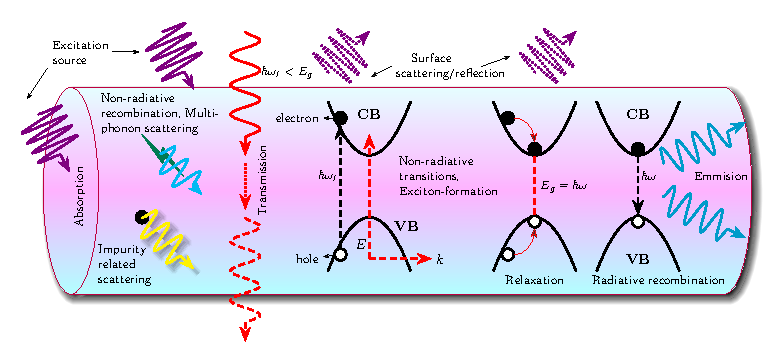
\includegraphics[width=0.8\linewidth]{FIGURES/Characterization_techniques/spectroscopies}
	\caption{Diagram showing the light-matter interaction for semiconductor nanostructures,the processes of emission, transmission, absorption and stattering can be observed.\cite{cardona2005fundamentals,yi2012semiconductor,sivadasan2017optical}}
	\label{fig:schematic-light-matter}
\end{figure}


\subsection{Ellipsometry (SE)}
\vspace{-1cm}
\lettrine[lines=3, lraise=0.1, nindent=0mm, slope=0mm]{\textbf{E}}{}llipsometry is an optical technique used for the characterization and observation of events in both an interface and a film, i.e. it takes advantage of the reflection or transmission of incident light from various materials that we wish to study. It is responsible for measuring the change of polarized light when reflecting or transmitting light in a sample and is called ellipsometry because the polarized incident light changes its polarization to elliptical after reflecting or transmitting in the sample,  It is widely used for its non-perturbing character \cite{azzam1978ellipsometry} (when the wavelength and intensity of the light beam are properly chosen) and in this sense, it can be measured in-situ and ex-situ, SE is highly sensitive to interfacial defects such as oxidation, evaporation of thin films among others\cite{fujiwara2007spectroscopic}.



\begin{figure}[H]
	\centering
	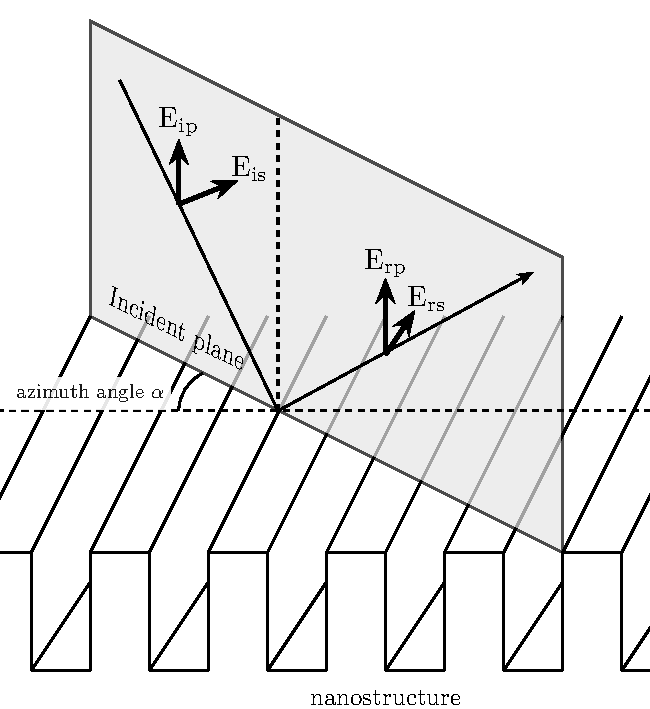
\includegraphics[width=0.5\linewidth]{FIGURES/Characterization_techniques/Nanostructure}
	\caption{Schematic of how light is reflected in a nanostructure, where Eip, Eis, Erp and Ers are the electromagnetic fields for incident and reflected light with polarization s and p respectively}
	\label{fig:sq-how to reflex}
\end{figure}

The interaction of the electric fields in a nanostructure and the distribution of the polarizations can be seen in Fig. \ref{fig:sq-how to reflex}. SE allows us to measure two fundamental values ($\psi$, $\Delta$) where $\psi$ represents the amplitude ratio and $\Delta$ refers to the phase difference between \textit{p} and \textit{s} polarization, this is done in a wavelength range in our case from $210$nm to $650$nm however, it can be done in the infrared range depending on the material under study and the properties of interest. \\
The reason for using SE in the developed work is to know the dielectric function of graphene, GNRs and CdTe-based materials as we can acquire information about the band structure and optical transitions \cite{fujiwara2007spectroscopic,weber2010optical}. \\

To understand this change of polarization when reflecting off the sample we can look at Fig. \ref{fig:ellips} where linearly polarized light is described as an electromagnetic wave with orthogonal electric \textbf{E} and magnetic \textbf{B} fields which are characteristic of light since it is a periodic transverse electromagnetic disturbance \cite{losurdo2013ellipsometry}. Linear polarization refers to the existence of an electric field orientation when the wave propagates in the $z$ direction, but the E field (and the B field) oscillates in x (and the B field in y), hence the transverse nature of light waves.  Circularly polarized light tells us that as the wave propagates the vector E rotates with the end point of the vector E tracing a circle, and for our case where the light is elliptically polarized hence an ellipse is shown as the projected locus of the end points of E as the wave propagates, but E also changes in magnitude and hence traces an ellipse. 

Therefore the polarization state is defined as follows: 

\begin{equation}
	\tan(\Psi)\epsilon^i\Delta)=a
\end{equation}

Where $r_s$ is the complex amplitude reflectance for the s-polarization, $r_p$ is the complex amplitude reflectance for the p-polarization, and $\Psi$ is the ellipsometric magnitude reflectivity ratio, and $\Delta$ is the ellipsometric phase term [80].

\begin{figure}[H]
	\centering
	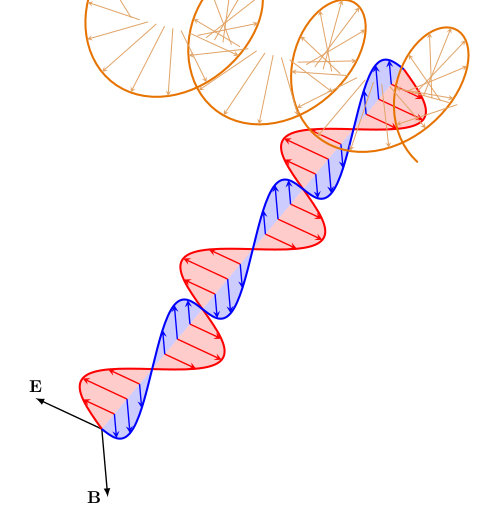
\includegraphics[width=0.5\linewidth]{FIGURES/Characterization_techniques/ellips-01.png}
	\caption{the waves}
	\label{fig:ellips}
\end{figure}

In order to obtain the experimental parameters we performed our experiments in a wavelength range from $210$nm to $650$nm  ($1.9$ev to $5.9$ev) in general, however we focus on the wavelength of our interest depending on the material under study. So spectroscopic ellipsometry is able to provide unique responses for material parameters (See.Fig \ref{fig:SE-surface})in addition to having a high have a sensitivity to material properties , it is worth mentioning that we can obtain both the real and imaginary part of the dielectric function without the need to perform KK analysis.\\


\begin{figure}[H]
	\centering
	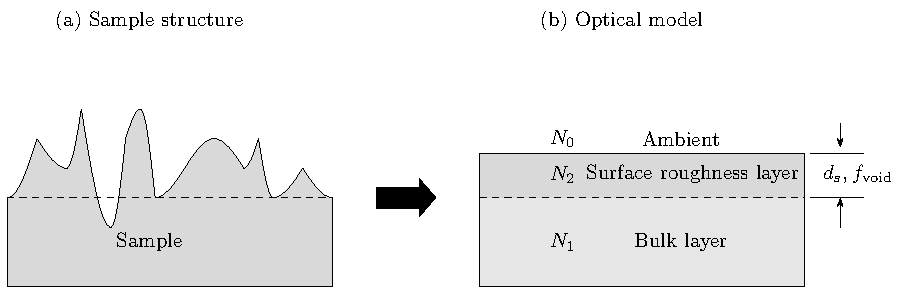
\includegraphics[width=0.8\linewidth]{FIGURES/Characterization_techniques/Surface-01}
	\caption{It can be seen a) sample with rough surface, b) optical model that is composed of the rough surface and the bulk layers, where $d_s and f$ are the thicknesses of the rough surface.}
	\label{fig:SE-surface}
\end{figure}

The photometric ellipsometer implemented at IICO (Instituto de Investigacion en Comunicacion Optica) has the RAE configuration which takes advantage of the modulation of the signal obtained thanks to a rotating analyzer, the array (see Fig. \ref*{fig:SE-SETUP-FINE} )starts with a $75$ W Xenon light source (Hammamatsu Photonics) and then passes through an array of mirrors (with focal length f/6) that lead to the monochromator (Jobin-Yvon-Spex with two diffraction gratings of 1200 lines/mm and 600 lines/mm) just in order to make the scan with monochromatic light,  then the collimated light thanks to a pair of mirrors (with focal length f/10) is directed through a linear polarizer (Rochon of \textit{Optics for Research}) which is at an azimuthal angle 30$\degree$ with respect to the angle of incidence and we focus it on the sample which is at an oblique angle of 70$\degree$, the reflection passes again through a linear analyzer (inverted polarizer) which is rotating at a fixed angular frequency of 856Hz, then this response is collected with a photomultiplier to measure the DC component we use a Keithley Multimeter 2000 multimeter and the AC signal is measured with a Lock-In amplifier Stanford Research System model SRS350. \\


\begin{figure}[H]
	\centering
	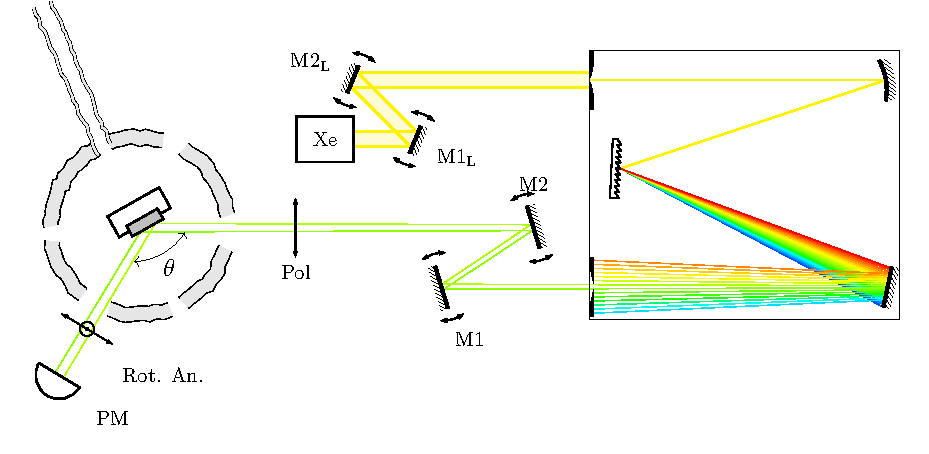
\includegraphics[width=0.85\linewidth]{FIGURES/Characterization_techniques/SE-SETUP-FINE}
	\caption{Schematic of SE coupled to a vacuum chamber used in this work, where XE is the xenon lamp, $M1_{L}$ and $M2_{L}$ corresponding to the first mirror array which incident the light at the entrance of the monochromator, at the output we have $M1$ and $M2$ then it passes through a polarizer with an angle of $\theta=30^{\circ}$, hits the sample inside the chamber with an angle of $\theta=64^{\circ}-70^{\circ}$ and its reflection, goes to the rotating polarizer and then the signal is detected by the photomultiplier}
	\label{fig:SE-SETUP-FINE}
\end{figure}

The acquired signals from both the multimeter and lock-in signals are processed with routines developed in Python so that the pseudo-dielectric function, absorption and layer thicknesses can be visualized. 

\subsection{Near-field scanning optical microscopy (NSOM)}
\vspace{-1cm}
Some of these SPM modes were SNOM (Scanning Nearfield Optical
Microscopy), but there are at least 20 different modes of AFM. SNOM is an example of
using the close contact and position control of the AFM to measure properties of the
surface other than topography (in this case, optical properties)

By combining optical spectroscopy with scanning near-field optical microscopy
(SNOM)


The Nanonics commercial system available at the IICO, mostrada , which was fundamental for the development of this work, has the capacity to make a scan to know the amount of reflected light and simultaneously know the morphology of the surface, that is to say, in a coupled AFM-NSOM way. We call the magnitude of the scans "windows" and they were studied from small areas $2\mu m \times 2\mu m$ to  $25\mu m \times 25\mu m$


\begin{figure}[H]
	\centering
	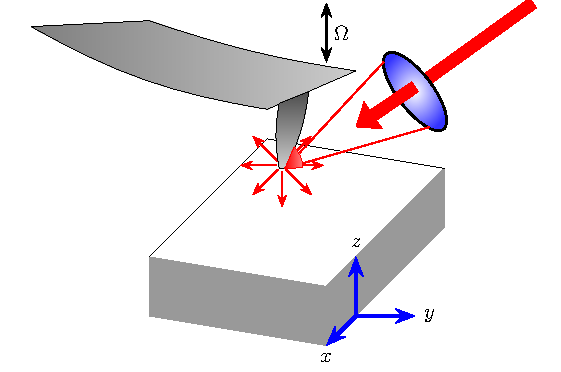
\includegraphics[width=0.7\linewidth]{FIGURES/Characterization_techniques/NSOM-setup}
	\caption{Schematic of }
	\label{fig:NSOM:SETUP}
\end{figure}





\subsection{Differencial Reflectance spectroscopy (RDS)}
\vspace{-1cm}
In the case of modulated spectroscopies these have been recognized to investigate optical properties that allow us to know the electronic structure of the material and therefore a variety of physical parameters. 

\begin{figure}[H]
	\centering
	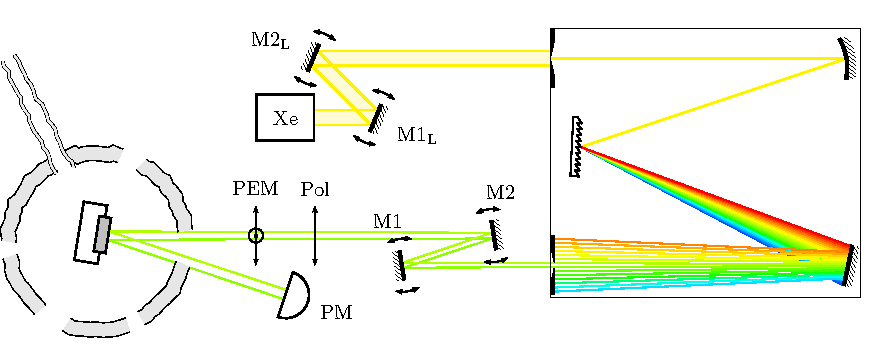
\includegraphics[width=1\linewidth]{FIGURES/Characterization_techniques/RAS-SETUP-FINE}
	\caption{Schematic of RDS coupled to a vacuum chamber used in this work, where XE is the xenon lamp, $M1_{L}$ and $M2_{L}$ corresponding to the first set of mirrors incident the light at the input of the monochromator, at the output we have $M1$ and $M2$ then it passes through a polarizer with an angle of $\theta=45^{\circ}$, impinges on the sample inside the chamber with an angle of $\theta=4.5^{\circ}$ and its reflection is detected by the photomultiplier.}
	\label{fig:ras-setup-fine}
\end{figure}



\section{Atomic Force Microscopy (AFM)}
\vspace{-1cm}
\lettrine[lines=3, lraise=0.1, nindent=0mm, slope=0mm]{\textbf{T}}{}o get into context about atomic force microscopy (AFM) \cite{binnig1982surface,binnig1986atomic} we must first describe the STM technique is based on studying the phenomenon of electron tunneling in conductive surfaces its inventors were \textit{G. Binning} and \textit{H. Rohrer} for which were awarded the Nobel Prize in Physics in 1986 and for such an interesting invention now have been investigated several metals and semiconductors \cite{cricenti2003afm,giessibl2003advances,zhong1993fractured} at the atomic scale which has allowed a series of advances in progress, a disadvantage that has the STM is that there needs to be electrical conduction in the samples (it's possible to obtain images of metals and conductive samples even HOPG but not in ambient conditions but in ultra-high vacuum environments\cite{nie1994atomic}) because the tunnel current flows between the tip and the sample, Even so, it was realized that if the distance between tip and the sample is very small the current can flow, and collateral forces are appreciated, this is where the search of\textit{Binning} comes in to apply it to insulating surfaces, so the AFM is developed, which is based on the repulsion force between tip and surface and no longer has the limitation of STM \cite{binnig1982surface}.\\

AFM was developed to start the principle of a measuring device, not only the forces arising from inter-atomic interactions, but also other forces such as those due to electric and magnetic fields\cite{binnig1986atomic}.


The principle of AFM in terms of surface "sensing" consists of a sharp tip on a cantilever (\textbf{\underline{See Fig. 1)}} to scan a specific area and due to the short range attractive forces between the surface and the tip causing it to flex to the surface as the approach increases, the repulsive forces also induce the tip to flex, the way in which these changes in tip deflection are detected in general is by incident a laser on the cantilever and the changes in the direction of the reflected beam translate into changes in the morphology of the sample under study.  \\
There are some ways in which morphology can be studied in AFM, in this case we will describe the contact mode and the tapping mode, this last way was the one used for the characterizations.

\subsection{Contact Mode} 
\vspace{-1cm}
\lettrine[lines=3, lraise=0.1, nindent=0mm, slope=0mm]{\textbf{T}}{}his mode can be considered standard and is a very powerful and used technique that consists of the tip being in contact with the surface and by repulsive force, the tip is deflected so that the respective topography is obtained, it is fast since it is not necessary to add the oscillation measurements and thus avoid time to obtain the image. 

However, there are some points to consider that in this mode i) given the repulsion between sample and tip, the sample can be damaged in the scan or the tip by abrupt changes in the scanning surface ii) because tip and sample are in constant contact in addition to the normal force applied between them, lateral forces are experienced \cite{eaton2010atomic, cricenti2003afm, aranha2018fabrication} 


\subsection{Tapping mode}
\vspace{-1cm}
\lettrine[lines=3, lraise=0.1, nindent=0mm, slope=0mm]{\textbf{T}}{}he tapping mode consists in that the cantilever vibrates at a resonance frequency in such a way that when approaching the sample, the tip slightly touches the surface in the final part of each oscillation, this is represented in a decrease of the amplitude and then with feedback cycle maintains this decrease in a preset value and the sweep is performed and in this way the topographic image of the surface is obtained, something that distinguishes it is that lateral forces are practically eliminated and the sample under study is not damaged\cite{putman1994tapping,cleveland1998energy}. 




\section{Raman spectroscopy}

\begin{figure}[H]
	\centering
	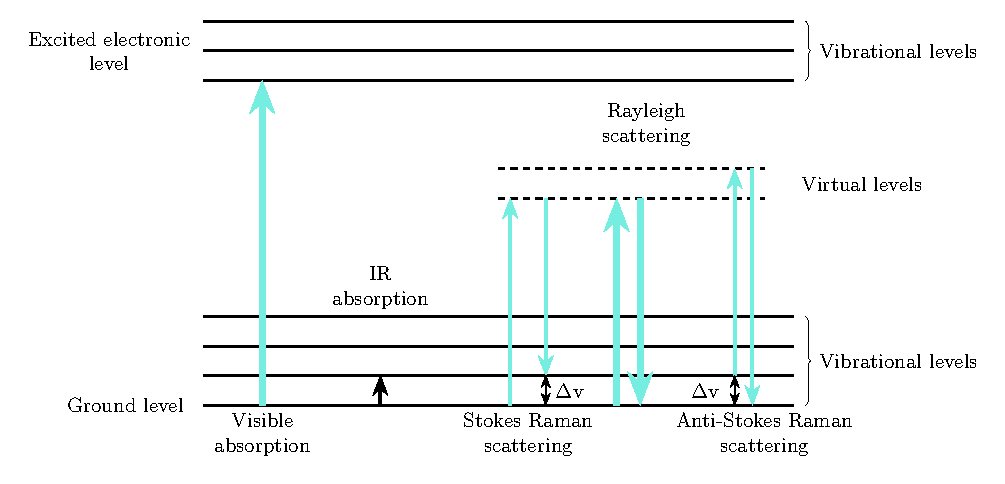
\includegraphics[width=0.85\linewidth]{FIGURES/Characterization_techniques/RAMAN-set}
	\caption{Schematic of RDS coupled to a vacuum chamber used in this work, where XE is the xenon lamp, $M1_{L}$ and $M2_{L}$ corresponding to the first set of mirrors incident the light at the input of the monochromator, at the output we have $M1$ and $M2$ then it passes through a polarizer with an angle of $\theta=45^{\circ}$, impinges on the sample inside the chamber with an angle of $\theta=4.5^{\circ}$ and its reflection is detected by the photomultiplier.}
	\label{fig:raman-set}
\end{figure}








\section{Samples Description}
\vspace{-1cm}
The studied samples described in the following table were synthesized at the Paul Drude Institute in Berlin, Germany by the group led by Dr. Marcelo Lopes. 

\newcolumntype{C}{>{\centering\arraybackslash}p{70mm}}% a centered fixed-width-column
\begin{table}[H]
	\centering
	\begin{tabular}{lCc}
		\hline
		\hline
		 &  Description &  Average width \\
		\hline
		FG163L &  QFS BL-GNRs on SI SiC(0 0 0 1) & $240 nm$\\
		FG166L &  QFS BL-GNRs on SI SiC(0 0 0 1) & $120 nm$\\
		FG166R &  QFS BL-GNRs on SI SiC(0 0 0 1) & $150 nm$\\
		FG271 &  ML-GNRs on buffer layer/SiC(0 0 0 1) & \\
		FG944&  QFS-BL-G on n-type SiC(0 0 0 1)       &  \\
		\hline
		\hline
	\end{tabular}
	\caption{Description of graphene and GNRS samples studied }
	\label{tab:CH 3 Section 3.1 Photodectors materials}
\end{table}

The development of non-invasive optical techniques for the study of various materials brings with it endless applications in the case of graphene in the field of electrinocs and microelectronics, 



y efectivamente se observa un cambio muy notorio en la respuesta de RDS en primera instancia esta se trato de emularla con un modelo de strain en la zona 
de alrededor 4ev, el s



El proceso para s

\begin{itemize}
	\item Limpieza de la muestra con tricloroetileno, enseguida enjuagar con 
	\item 
\end{itemize}
Las transiciones localizadas en 2.5ev y 4ev muestran un cambio incluso la forma de linea tiene una evolucion maximizando estas donde se observa por una parte que se tiene un deposito de Ag e incluso se puede modelar con la funcion dielectrica que se obtiene antes y despues de los depositos, tal como comenta el diagrama en la parte tecnica de la misma se puede obtener diversas propiedades con esta forma de linea tanto del espesor de las peliculas como espesor de los oxidos que se crecen sobre la muestra


En el caso de las muestras de grafeno, descritas como los nanolistones se puede observar que podemos tanto obtener informacion de las capas de las cuales estan compuestas como de la resolucion lateral d ela misma. 
La resolucion que nos brinda NSOM nos permite tanto obtener informacion estructural como optica, al estar haciendno incidir sobre la punta de NSOM e ir barriendo, la comparacion o el tranlape que se puede hacer es bastante util por que nos damos cuenta que realizando un modelo de tres capas de la reflectividad donde se involucran los coeficientes de reflexion de fresnel los cuales se explican en la parte teorica de la misma podemos entender como un sistema de silicio, oxido de silicio, multiples capas de  de grafeno y aire, simepre los medios superiores e inferior los consideramos como infinitos con el fin de mantener aislado en sistema y que nos pueda brindar una mejor respepuesta y mas cercana a la real que vemos de manera experimental,  en el caso de las muestras exfoliadas y en el caso de los nanolistines de grafeno tenemos carburo de silicio en su forma hexagonal para de esta forma sintetizar el grafeno ya uqe su configuracion crsitalina es hexagonal, la manera en la uqe se sinbtetiza y fue descrita en la parte de muestra se puede apreciar que la terminacion en los bordes del edge de los escalones se suelen aculumar demasiado que os brinda incluso en muchos casos multiples monocapas de grafeno, tal como se menciona en una manera comun del crecimiento, sin embargo con todas las condiciones esperadas podemos tener un crecimento controlado.

